\documentclass[
    10pt,
    aspectratio=169,
    xcolor={dvipsnames},
    spanish,
    % handout,
    % notes=only,
    % notes,
    ]{beamer}

% BEAMER SETTINGS
\setbeamerfont{section in toc}{size=\normalsize, shape=\bfseries}
\mode<presentation>{
    \usetheme{Antibes}
    \setbeamercovered{transparent}
    \usecolortheme{rose}
    \setbeamertemplate{navigation symbols}{}
    }

% PACKAGES
% \usepackage[spanish]{babel}  % uncomment for Spanish support
\usepackage{tikz,pgfplots}
\pgfplotsset{compat=1.13}
\usetikzlibrary{calc}
\usepackage{subcaption}
\usepackage{graphicx}
\graphicspath{{figures/}}
\usepackage{booktabs}
\usepackage{upgreek}
\usepackage{commath}
\usepackage{amsmath,amsthm,amssymb,mathtools,mathrsfs}
\usepackage{cancel}
\usepackage{fontawesome5}
\usepackage{enumerate}
\usepackage{tensor}
\usepackage[font=footnotesize]{caption}
\usepackage{wasysym}

\usepackage[skins,theorems]{tcolorbox}
\tcbset{
    highlight math style={
        enhanced,
        coltext=black,
        colframe=black,
        colback=lightgray,
        arc=0pt,
        boxrule=.5pt
        }
}

% REFERENCES AND OTHERS
\usepackage{aas_macros}
\usepackage{natbib}
\bibpunct{(}{)}{;}{a}{}{,}

\usepackage{siunitx}
\sisetup{
    range-phrase=\text{--},
    range-units=single,
    separate-uncertainty=true,
    print-unity-mantissa=false
    }
\DeclareSIUnit{\gauss}{G}
\DeclareSIUnit{\jansky}{Jy}
\renewcommand{\figurename}{Fig.}

\usepackage{hyperref}
\hypersetup{
    % bookmarks=true,
    unicode=true,
    pdftoolbar=true,
    pdfmenubar=true,
    pdffitwindow=false,
    pdfstartview={FitH},
    pdftitle={ISI-Free Linear Combination Pulses with Better Performanc},
    pdfauthor={Erik Saez A.},
    pdfcreator={Erik Saez A.},
    pdfnewwindow=true,
    colorlinks=true,
    linkcolor=RoyalBlue,
    citecolor=RoyalBlue,
    urlcolor=RoyalBlue
    }

\title[Auxiliar \#4 - Ondas ondas ondas]{\bfseries Auxiliar \#4 - Ondas ondas ondas}
\subtitle{Introducción a la Física Moderna (F1100-5) (Mejor Sección!!)}
\author[Erik Saez A.]{Erik Saez A. - Javiera Toro}
\institute[UChile]{Departamento de Ingeniería Eléctrica \\ Universidad de Chile}

\date{\today}

\begin{document}

\begin{frame}
  \titlepage
  \centering
  \faIcon{envelope} \href{mailto:erik.saez@ug.uchile.cl}{erik.saez@ug.uchile.cl} \hspace{.2cm}
\end{frame}

\begin{frame}{Contenidos}
  \tableofcontents
\end{frame}

\section{Resumen}

% ====== Frame 1: MAS (distribución 2x2, compacto y simétrico) ======
\begin{frame}{M.A.S.: Ecuación y Solución}
  \footnotesize
  \begin{columns}[T]
    \begin{column}{0.58\textwidth}
      \begin{block}{EDO del M.A.S.}
        Una \textbf{ecuación diferencial ordinaria (EDO)} relaciona una función   desconocida y sus derivadas respecto de una sola variable independiente. La forma más común que encontraremos es la EDO lineal homogénea de 2° orden:
        \begin{equation*}
          m\ddot x + kx = 0 \;\Longleftrightarrow\; \ddot x + \frac{k}{m}x = 0
        \end{equation*}
        \noindent Frecuencia angular $\omega^2=\tfrac{k}{m} \;\Rightarrow\; \omega=\sqrt{\tfrac{k}{m}}$, que cuantifica la rapidez de la oscilación.\vspace{-2pt}
      \end{block}
      \begin{block}{Posición de equilibrio}
        La \textbf{posición de equilibrio} $x_{\text{eq}}$ es aquella en la que la fuerza neta (y por ende la aceleración) se anula: $m\ddot x=0$, lo que implica que:\begin{align}
          \ddot{x}= \dot{x} = 0
        \end{align}
      \end{block}
    \end{column}
    \begin{column}{0.45\textwidth}
      \begin{block}{Derivadas útiles}
        Cambio de variable respecto al equilibrio:\\[-2pt]
        \[
          \begin{aligned}
            y(t) &= x(t)-x_{\text{eq}},\\
            \dot y(t) &= \dot x(t),\\
            \ddot y(t) &= \ddot x(t).
          \end{aligned}
        \]
      \end{block}
      \begin{block}{Solución general y derivada (conocida)}
        Para $\ddot x + \omega^2 x=0$:
        \[
          \begin{aligned}
            x(t) &= A\cos(\omega t)+B\sin(\omega t),\\
            \dot x(t) &= -A\omega\sin(\omega t)+B\omega\cos(\omega t).
          \end{aligned}
        \]
        C.I.: $x(t= 0)=x_0 \Rightarrow A=x_0$, $\;\dot x(0)=v_0 \Rightarrow B=v_0/\omega$.
      \end{block}
    \end{column}
  \end{columns}
\end{frame}

% ====== Frame 2: Ondas: viajeras y superposición (2x2 equilibrado) ======
\begin{frame}{Ondas en cuerdas: viajeras y superposición}
  \footnotesize
  \begin{columns}[T,totalwidth=\textwidth]
    % ---------- Columna izquierda ----------
    \begin{column}{0.4\textwidth}
      \begin{block}{Ecuación de onda y velocidad}
        La ecuacion de la onda describe el comportamiento temporal y espacial de perturbaciones que se propagan en un medio.
   
        \[
          \frac{\partial^{2}y}{\partial t^{2}}
          = c^{2}\,\frac{\partial^{2}y}{\partial x^{2}},
          \qquad c=\sqrt{\tfrac{T}{\rho}}.
        \]
    
      \end{block}
      \begin{block}{Soluciones de d’Alembert}
        La solucion de la ecuación de onda es:
    
        \[
          y(x,t)=f(x-ct)+g(x+ct).
        \]
        \begin{itemize}
          \item \textbf{Derecha:} $f(x-ct)$ (traslación en $+x$).
          \item \textbf{Izquierda:} $g(x+ct)$ (traslación en $-x$).
        \end{itemize}
     
      \end{block}
    \end{column}
    % ---------- Columna derecha ----------
    \begin{column}{0.5\textwidth}
      \begin{block}{Onda armónica viajera}
       
        \begin{align}
          y(x,t)=A\cos(kx-\omega t+\phi)\\
          k=\tfrac{2\pi}{\lambda},\quad c=\tfrac{\omega}{k}=\tfrac{\lambda}{T}
        \end{align}
          
      \end{block}
      \begin{block}{Superposición / Interferencia (misma $k,\omega$)}
      
        \[
          y_1=A\cos\Theta,\quad
          y_2=A\cos(\Theta+\Delta\phi),\qquad
          \Theta=kx-\omega t+\phi.
        \]
        Suma:
        \[
          y=y_1+y_2=
          2A\cos\!\Big(\tfrac{\Delta\phi}{2}\Big)\,
          \cos\!\Big(\Theta+\tfrac{\Delta\phi}{2}\Big).
        \]
        Casos clave:
        \begin{itemize}
          \item \textbf{En fase} ($\Delta\phi=0$): amplitud $=2A$ (constructiva).
          \item \textbf{En contrafase} ($\Delta\phi=\pi$): amplitud $=0$ (destructiva).
        \end{itemize}
  
      \end{block}
    \end{column}
  \end{columns}
\end{frame}



% ===================================

% =====================================
\section{Pregunta 1}

% ------------------ Ejercicio 1 ------------------
\begin{frame}{Ejercicio 1}
  \begin{columns}[T,totalwidth=\textwidth]
    \begin{column}{0.6\textwidth}
      \begin{block}{Enunciado pregunta 1}
        \footnotesize
        Una partícula de masa $m$, después de caer una distancia $h$, se adosa a un resorte (largo) de constante $k$.
El sistema resultante viene gobernado por la ecuación de movimiento
\begin{equation}
  \ddot z + 2\omega_0 \dot z + \omega_0^{2}\, z \;=\; 0,
  \label{eq:crit}
\end{equation}
donde la magnitud $z(t)$ mide la posición de la partícula respecto del punto de equilibrio y
$\omega_0=\sqrt{k/m}$ es la frecuencia natural del sistema. La solución general está dada por
\begin{equation}
  z(t) \;=\; \big(A + B\,t\big)\,e^{-\omega_0 t}.
\end{equation}

\begin{enumerate}
  \item Determine $A$ y $B$ usando las condiciones iniciales.
  \item Sea $t_0$ el instante en que el resorte tiene su máxima compresión. Evalúe $t_0$
  (elija el cero del tiempo en el instante en que la partícula colisiona con el resorte).
  \item Haga un gráfico esquemático de la función $z(t)$.
\end{enumerate}
      \end{block}
    \end{column}
    \begin{column}{0.40\textwidth}
      \centering
       \vspace*{1cm}
      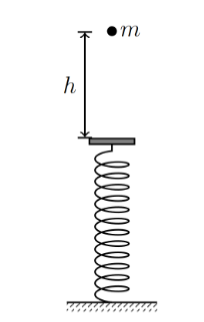
\includegraphics[width=0.6\textwidth]{Auxiliar_2_9.png}
    \end{column}
  \end{columns}
\end{frame}
\section{Pregunta 2}

%-------------------------------------
\begin{frame}
  
\end{frame}
% ------------------ Ejercicio 2 ------------------
\begin{frame}{Ejercicio 2}
  \begin{block}{Enunciado pregunta 2}
    Se tiene una cuerda muy larga de tensión $T=1\,\mathrm{N}$ y densidad lineal $\rho=0.25\,\mathrm{kg/m}$.
El extremo izquierdo de la cuerda se mueve de la siguiente forma:
\begin{enumerate}
  \item Está quieto hasta $t=0$.
  \item Desde $t=0\,\mathrm{s}$ hasta $t=2\,\mathrm{s}$, sube con velocidad constante de $1\,\mathrm{cm/s}$.
  \item Luego, se mantiene quieto por $1\,\mathrm{s}$.
  \item Finalmente, baja a velocidad constante hasta la posición inicial, tardando $1\,\mathrm{s}$ en ello.
\end{enumerate}
Grafique el perfil de la onda para $t=3\,\mathrm{s}$.
  \end{block}

\end{frame}
\section{Pregunta 3}
% ------------------ Ejercicio 3 ------------------
\begin{frame}{Ejercicio 3}
  \footnotesize
  \begin{columns}[T,totalwidth=\textwidth]
    \begin{column}{0.58\textwidth}
      \begin{block}{Enunciado Pregunta 3}
      Se tiene una cuerda ideal, sobre la que pasa una onda armónica transversal (el desplazamiento de la cuerda es paralelo al eje $y$ y la onda viaja en el eje $x$). El lado izquierdo (a) de la figura muestra, en función del tiempo, el movimiento de un trozo infinitesimal de la cuerda ubicado en $x=5~\text{m}$.

\begin{enumerate}
  \item Uno de los cuatro gráficos de posición $y$ vs.\ $x$ en la parte derecha (b) de la figura representa una \emph{“foto”} de la onda en un instante en el tiempo (el momento en el tiempo para cada caso se indica en el gráfico). Encuentre cuál gráfico $y$ vs.\ $x$ pertenece a la onda mostrada en el lado izquierdo. Justifique su respuesta.

  \item Determine la amplitud, longitud de onda y período de la onda. Explique cómo deduce estos valores.

  \item Encuentre la rapidez a la que viaja la onda.

  \item Encuentre la dirección (derecha o izquierda) en que se mueve la onda. Justifique su respuesta.
\end{enumerate}
      \end{block}
    \end{column}
    \begin{column}{0.40\textwidth}
      \centering
  \vspace*{1cm}
      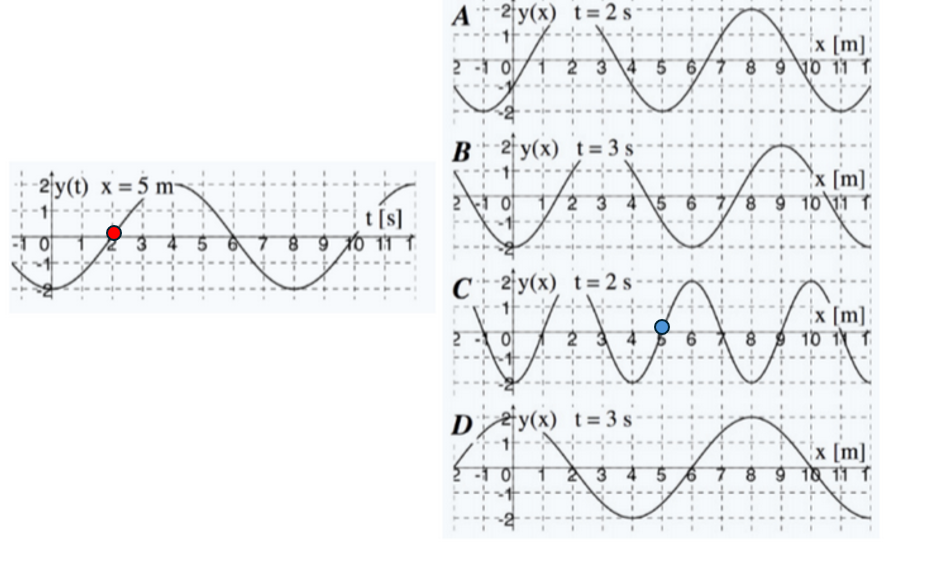
\includegraphics[width=1.3\textwidth]{Auxiliar_2_12.png}
    \end{column}
  \end{columns}
\end{frame}
%--------------------------------------------
\begin{frame}{Ejercicio 4}
  \begin{columns}[T,totalwidth=\textwidth]
    \begin{column}{0.58\textwidth}
      \begin{block}{Enunciado Pregunta 4}
     Considere una cuerda de densidad lineal $\rho$ y largo $L$ que se cuelga del techo
sin sostener ninguna masa, como se indica en la figura. Se golpea la cuerda en el
centro generando dos pulsos que se propagan, uno ascendente y otro descendente.

\begin{enumerate}
  \item ¿Cuál de los pulsos llegará primero al extremo correspondiente de la cuerda?
  \item Al llegar al respectivo borde, cada pulso será reflejado. Diga si los pulsos se reencontrarán en el centro de la cuerda, por encima o por debajo del mismo. ¿Cómo será la superposición de los pulsos en ese instante?
\end{enumerate}
      \end{block}
    \end{column}
    \begin{column}{0.50\textwidth}
      \centering
  % bajar solo la imagen de la Pregunta 3
  \vspace*{1cm}
      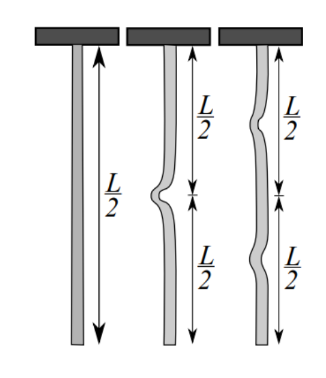
\includegraphics[width=0.7\textwidth]{Auxiliar_2_3.png}
    \end{column}
  \end{columns}
\end{frame}
%----------------------------
\begin{frame}{Ejercicio 5}
  \footnotesize
  \begin{columns}[T,totalwidth=\textwidth]
    \begin{column}{0.58\textwidth}
      \begin{block}{Enunciado Pregunta 5}
    Los planetas del sistema solar poseen muchos más tipos de movimientos que el de rotación y el de traslación, algunos de ellos muy complejos, con períodos muy cortos, muy largos o incluso erráticos. Debido a la estabilidad de las órbitas alrededor del Sol, los planetas pueden describir movimientos oscilatorios en el eje radial; es posible ver un ejemplo de esto usando simples aproximaciones.

Se tiene un planeta de masa $m$ que realiza una órbita circular de radio $R_0$ alrededor de una estrella de masa $M$. Considere ahora que la órbita del planeta es ligeramente perturbada, tal que el momento angular de la órbita no cambia, pero sí su radio en una pequeña cantidad. Usando aproximaciones adecuadas, muestre que el radio de la órbita del planeta está descrito por un oscilador armónico.
      \end{block}
    \end{column}
    \begin{column}{0.40\textwidth}
      \centering
  % bajar solo la imagen de la Pregunta 3
  \vspace*{1cm}
      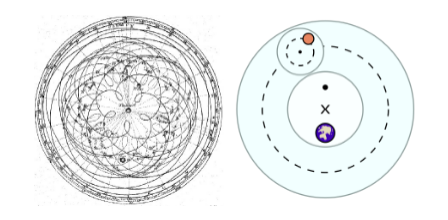
\includegraphics[width=1\textwidth]{Auxiliar_2_10.png}
    \end{column}
  \end{columns}
\end{frame}



\end{document}
